\section{System Implementation}
\label{clicknp:sec:impl}

\subsection{\name Toolchain and Hardware Platform}

This chapter implements a \name compiler as the front end of the \name toolchain (\S \ref {clicknp:subsec:toolchain}).
For the host program, Visual C++ is utilized as the backend. Further integration of the Altera OpenCL SDK (i.e., Intel FPGA SDK for OpenCL) \cite {aoc} and Xilinx SDAccel \cite {vivado} as the backend for FPGA programs.
The core part of the \name compiler contains about 20,000 lines of C++, flex, and bison code, which parse configuration files and component declarations, perform the optimizations described in Section \ref {clicknp:sec:optimization}, and generate code specific to each commercial high-level synthesis tool.

For components running on the FPGA, each component is compiled into intermediate C code, which is then compiled into a logic module by a high-level synthesis tool.
When using the Altera OpenCL high-level synthesis tool, each \name component is compiled into a \textit {kernel}, the connections between components are compiled into Altera extended channels (channel), which are then implemented with the Avalon ST interface; the components communicate with the on-board DRAM (i.e., global memory) using the Avalon MM interface.
When using the Xilinx SDAccel high-level synthesis tool, each component is compiled into an IP core, and the connections between components are implemented using AXI streams, and the AXI memory-mapped interface is used to access the on-board DRAM.
Components running on the host are compiled into CPU binary files, and the management process creates a worker thread for each host component.
Each pipeline between the host and FPGA components is mapped to a \textit {slot} of the PCIe I/O channel (\S \ref {clicknp:subsec:pcie}).

The hardware platform of this paper is based on the Altera Stratix V FPGA and Catapult shell \cite {putnam2014reconfigurable}.
The Catapult shell also includes an OpenCL-specific runtime (BSP). \name user logic communicates with the shell through the BSP.
\name user logic runs in an independent clock domain, and the BSP converts interfaces such as PCIe DMA and DRAM in the shell in different clock domains to the user logic's clock domain through asynchronous FIFO.
The BSP also provides management functions such as OpenCL kernel start and stop.
At the time of writing this paper, the author has not yet obtained the Xilinx hardware platform.
Therefore, the system evaluation is mainly based on the Altera platform using \name + OpenCL, and the reports generated by Vivado HLS (such as frequency and area costs) are used to understand the performance of \name + Vivado.

\subsubsection{Intermediate C Code Suitable for High-Level Synthesis Tools}

Upon powering on the host or online reconfiguration of the FPGA, each kernel or IP core commences parallel operation. As depicted in Figure \ref{clicknp:fig:intermediate-c}, each kernel initially executes the initialization (init) function, then enters an infinite loop, checks the input pipeline and executes the event handling (handler) function, checks the signal and executes the event handling function.

\begin{figure}[htbp]
	\small
	\centering
	\begin{tabular}{c}
\begin{lstlisting}
void kernel() {
  Call init function;
  Declare and initialize input and output buffers;
  while (true) {
    if (input buffer is free and input pipeline is not empty) {
      Move data from input pipeline to input buffer;
    }
    Call handler function;
    if (output pipeline is free or output buffer is full) {
      Move data from output buffer to output pipeline;
    }
    if (input event pipeline is not empty) {
      Read input event from input event pipeline;
      Call signal function;
      Write event handling response to output event pipeline;
    }
  }
}
\end{lstlisting}
	\end{tabular}
	\caption{Pseudocode of Kernel Intermediate C Code.}
	\label{clicknp:fig:intermediate-c}
\end{figure}

High-level synthesis tools convert the intermediate C code into a hardware description language. Each loop in the intermediate C code is either fully unrolled into a pipelined logic module or implemented as a state machine, with each clock cycle executing one iteration of the loop. Loop unrolling is only applicable when the number of loop iterations is statically known at compile time and the number of iterations is small. For loops implemented as state machines, there may be data dependencies between different iterations of the loop, and the pipelined logic of one iteration may take several clock cycles to complete, so there may be several clock cycles of interval between two consecutive loop iterations. High-level synthesis tools need to calculate the minimum interval (initiation interval, II) between two consecutive iterations based on dependency relationships and pipeline delay information of the loop body. The smaller the II, the higher the throughput. Therefore, we aim to minimize II as much as possible.

Currently, high-level synthesis tools are primarily designed for compute-intensive operations. These operations often consist of multi-level nested loops, and the loop transformation methods used by compilers are typically applicable to programs with static control parts and perfectly nested loops during control flow compilation. However, the number of times the while loop in the program in Figure \ref{clicknp:fig:intermediate-c} is executed is unknown at compile time, and due to the presence of input/output buffer movement code, the loops in the handler and signal functions are not perfectly nested loops. Early versions of high-level synthesis tools may not only fail to compile, take too long to compile, and other errors for more complex source programs due to completeness issues, but also analyze too many unnecessary memory dependencies, leading to a large II, or even cause II static analysis failure, and the inner loop cannot be parallelized.

This paper aims to circumvent the nested loop optimization of existing high-level synthesis tools. Observing that the component calculation logic in network functions is relatively simple, and the amount of data processed per clock cycle is also very limited (such as one flit), many loop execution times can be statically determined at compile time (for example, processing each byte of a flit). Therefore, \name unrolls or flattens all loops in the handler and signal functions, so that the generated intermediate C code only has a while loop, and there are no nested loops, as shown in Figure \ref{clicknp:fig:flatten}. The default strategy of \name is to unroll loops that can be determined at compile time and flatten all other loops. Users can also specify the unrolling and flattening strategy through compilation options (pragma) embedded in the source program. In this way, high-level synthesis tools only need to analyze a single loop, reducing the possibility of errors.

Unrolling the loop body also has a significant advantage: it facilitates compiler optimization. Traditional compilers often find it difficult to optimize vector operations represented by loops. After \name unrolls the loop, the vector operation is decomposed into point-by-point operations, and high-level synthesis tools can perform a series of optimizations such as constant propagation and dead code elimination. In addition, after unrolling the loop, \name can perform static single assignment transformation, and can also expand the array with access addresses determined by loop variables into several discrete registers, thereby eliminating memory dependencies.

The \name can generate performance analysis reports. Within each component, the analysis report includes the storage method of each variable, the unrolling or flattening strategy of each loop, the minimum interval (II) between two adjacent iterations, and the dependency chain causing the II bottleneck. At the computational graph level, the analysis report includes the delay, throughput, and clock frequency of each component.

\begin{figure}
	\lstset{style=numbers}
	
	\centering
	\renewcommand{\baselinestretch}{0.75}
	\begin{tabular}{c}
		{
			\small
\begin{lstlisting}[escapechar=@]
while (true) {
  Packet pkt = read_input_port(in);
  uchar checksum = 0;
  #pragma unroll 2
  for (int i = 0; i < pkt.num_flits(); i++) {
    flit f = pkt.filt(i);
    for (int j = 0; j < FLIT_BYTES; j++)
      checksum ^= f.bytes[j];
  }
  write_output_port(out, checksum);
}
\end{lstlisting} 
		} \\
		(a) Original C intermediate code (schematic code).  \\
		{
			\small 
\begin{lstlisting}[escapechar=@]
uchar checksum = 0;
Packet pkt;
int i = 0;
while (true) {
  if (i == 0)
    pkt = read_input_port(in);
  if (i < pkt.num_flits()) {
    flit f = pkt.filt(i);
    checksum ^= f.bytes[0]; checksum ^= f.bytes[1];
    ...
    checksum ^= f.bytes[FLIT_BYTES - 1];
    i++;
  }
  if (i < pkt.num_flits()) {
    flit f = pkt.filt(i);
    checksum ^= f.bytes[0]; checksum ^= f.bytes[1];
    ...
    checksum ^= f.bytes[FLIT_BYTES - 1];
    i++;
  }
  if (i == pkt.num_flits()) {
    write_output_port(out, checksum);
    i = 0;
  }
}
\end{lstlisting} 
		} \\
		(b) The result after loop unrolling and flattening.
	\end{tabular}
	\caption{Loop unrolling and flattening. The i loop is unrolled according to the parallelism 2 and flattened; the j loop is fully unrolled: the result of the transformation is that all bytes of 2 flits are calculated per clock cycle.}
	\label{clicknp:fig:flatten}
\end{figure}

\subsubsection{Optimization of Compilation Speed}

One limitation of FPGA programming is the relatively long compilation time. A simple network packet forwarding function requires about 3 hours to compile. The compilation time is mainly composed of several stages such as high-level synthesis, IP core generation, hardware description language logic synthesis, FPGA layout routing, and timing analysis.
This chapter adopts several techniques to shorten the FPGA compilation time.
First, the OpenCL programming framework generates IP cores from the Verilog modules generated by high-level synthesis and inserts them into the shell part, which requires copying a large amount of IP core and shell part code. Noting that the peripheral interface of user logic is fixed, this paper pre-generates IP cores and only needs to replace the high-level synthesis Verilog module files into the project; for the shell part code, file references are used instead of copying.
Second, in order to shorten the logic synthesis time, the fixed shell part is synthesized into a netlist file through logic synthesis, and the synthesis result is retained by using design partition, which can reduce the logic synthesis time of the shell part by about 35 minutes.
Third, in order to speed up the convergence speed of the FPGA layout algorithm, after the initial compilation is completed, the layout constraints of each module of the shell part are added to basically fix its layout. Most of the modules in the shell part interact with the hard IP at fixed positions on the chip, so it is reasonable to fix the layout near the hard IP. However, for better performance, this paper does not use design partitions to completely fix the layout and routing of the shell part. This optimization can save about 20 minutes.
Fourth, distinguish between debug and release compilation modes. The debug mode aims to verify the correctness of the logic, not to pursue performance. In debug mode, the clock frequency of user logic is fixed at 50~MHz, which greatly reduces the difficulty of layout and routing; the layout and routing of the shell part are solidified using design partitions, and the layout and routing of this part of high-frequency logic takes a long time. The debug mode can save 25 minutes of compilation time compared to the release mode, and more time will be saved when the user logic is more complex.
Fifth, unnecessary timing analysis models are deleted. The OpenCL framework defaults to analyze timing constraints under four conditions, but as long as the most stringent one is met, the other three can also be met, so we only retain the most stringent timing constraint model.
Sixth, in order to achieve the highest possible performance, the OpenCL framework first compiles with a higher user logic clock frequency (such as 250~MHz), then calculates the longest delay and the highest clock frequency that can work correctly based on the timing analysis results, and then uses this clock frequency for secondary layout and routing and timing analysis. This can achieve the highest possible throughput for compute-intensive workloads. However, this paper focuses on network packet processing, and only needs to achieve network line speed processing capabilities, so it can fix the clock frequency at 180 MHz, most user logic can reach this frequency, so there is no need to re-layout and route.

\begin{table}[htbp]
	\centering
	\caption{FPGA compilation acceleration technology.}
	\label{clicknp:tab:fpga-compilation}
	\small
	\begin{tabular}{l|p{.4\textwidth}|p{.15\textwidth}|p{.15\textwidth}}
		\toprule
		Compilation stage & Optimization method & Compilation time before optimization (min) & Compilation time after optimization (min) \\
		\midrule
		ClickNP compilation & -- & 0.1 & 0.1 \\
		High-level synthesis & -- & 1 & 1 \\
		Generate IP core & Pre-generate IP core; use file reference instead of copying & 10 & 0 \\
		Logic synthesis & Retain the synthesis result of the shell & 50 & 15 \\
		Layout and routing & Add layout constraints of the shell; in debug mode, lower the clock frequency of user logic, retain the layout and routing results of the shell & 60 & 40 (15)* \\
		Timing analysis & Delete unnecessary timing analysis models & 15 & 5 (0)* \\
		Secondary layout and routing & Fix the clock frequency, no need to re-layout and route & 30 & 0 \\
		Secondary timing analysis & Delete & 15 & 0 \\
		\midrule
		Total & -- & 180 & 60 (30)* \\
		\bottomrule
		\multicolumn{4}{l}{* The number in parentheses is the compilation time in debug mode.}
	\end{tabular}
\end{table}

Table \ref{clicknp:tab:fpga-compilation} summarizes the above compilation acceleration techniques. Before optimization, developers could only debug 3 rounds per working day, but after optimization, they can debug about 10 rounds in debug mode, and system tests that require performance can also be conducted about 6 rounds, greatly improving work efficiency.


\subsection{\name Component Library}
\label{clicknp:subsec:lib}

This paper implements a \name{} component library containing nearly 200 components.
Some of them (about 20%) come directly from the Click Modular Router, but are rewritten using the \name{} programming framework.
These components cover a large number of basic operations of network functions, including packet parsing, checksum calculation, encapsulation/decapsulation, hash table, longest prefix matching (LPM), rate limiting, encryption, and packet scheduling.
Due to the modular architecture of \name, the code size of each component is moderate.
The average line of code (LoC) of the components is 80, and the most complex component \textit {PacketBuffer} has 196 lines of C code\footnote{The number of lines of code refers to the \name component code, excluding the host control program and test code.}.

The table referred to as \ref {clicknp:tab:elements} showcases a selection of key elements implemented in \name. Along with the name of each element, the table also denotes the demo network functions that employ each element (these are elaborated further in section \ref {clicknp:sec:application}). The optimization techniques previously discussed in section \ref {clicknp:subsec:paral_in_elem} are utilized to minimize memory dependencies and balance pipeline stages. The third column of the table provides a synopsis of the optimization techniques employed by each element. 

For the elements listed at the top of Table \ref {clicknp:tab:elements}, the processing logic within the elements necessitates access to every byte of the packet. The throughput for these elements is provided in Gbps. However, the elements listed at the bottom of the table only process packet headers (metadata), hence it is more suitable to measure their throughput in packets per second. It is crucial to note that the throughput measured in Table \ref {clicknp:tab:elements} represents the maximum throughput that the corresponding elements can attain. When these elements are employed in real network functions, other components, such as Ethernet ports, may become the bottleneck. 

For reference, Table \ref {clicknp:tab:elements} compares the optimized FPGA version, a simple FPGA implementation that does not apply the techniques described in section \ref {clicknp:sec:optimization}, and a CPU implementation. The table clearly demonstrates that, post optimization, all of these elements can process packets very efficiently, achieving speeds that are 7 to 117 times faster than the initial FPGA implementation and 21% faster than a software implementation on a CPU core. This enhancement in performance is attributed to the ability to exploit the massive parallelism offered by the FPGA. 

Considering the power consumption of the FPGA (approximately 30W) and the CPU (approximately 5W per core), the energy efficiency of the \name elements is 4 to 120 times greater than that of the CPU. Table \ref {clicknp:tab:elements} also provides information on the processing delay of each element. As can be observed, this delay is very low, with an average of $0.19 \mu s$ and a maximum of only $0.8 \mu s$ (LPM \_Tree).

The final two columns of the table provide a summary of the resource utilization of each element, with utilization normalized to the capacity of the FPGA chip. Most elements only use a small number of logic elements, which is to be expected given that most packet operations are simple. The HashTCAM and RateLimiter elements have moderate logic resource usage due to their larger arbitration logic. However, BRAM usage largely depends on the configuration of the element. For example, the rate of BRAM usage increases linearly with the number of entries supported in the flow table. 

In summary, the FPGA chip used in this study has sufficient capacity to support meaningful network functions that contain a small number of elements.

\subsection{PCIE I/O Channel}
\label{clicknp:subsec:pcie}

As previously stated, a key characteristic of \name is its support for combined CPU / FPGA processing. This chapter accomplishes this objective by designing a high-throughput, low-latency PCIe I / O channel. \name supports flexible I/O operations. As depicted in Figure \ref{clicknp:fig:pcie-io}, \name offers two abstractions for communication with the host CPU based on slots and work queues, and also provides an interface for raw DMA operations.

\begin{figure}[htbp]
	\centering
	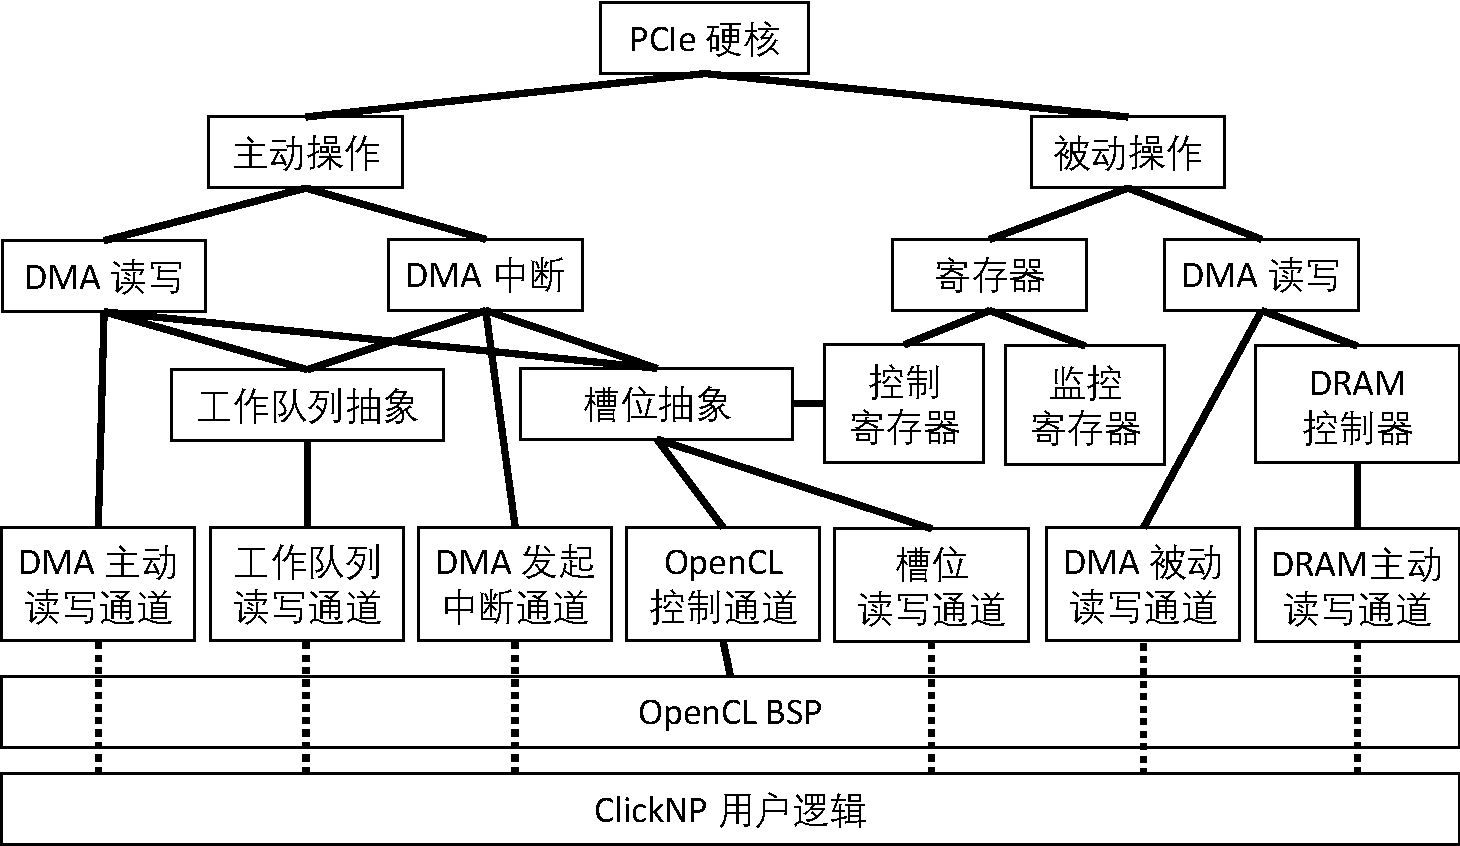
\includegraphics[width=0.8\textwidth]{image/pcie-io}
	\caption{Architecture of the PCIe I/O channel.}
	\label{clicknp:fig:pcie-io}
\end{figure}

In the slot-based abstraction, the PCIe physical link is divided into 64 logical sub-channels, or \textit {slots}. Each slot has a pair of send and receive buffers for DMA operations. Of the 64 slots, 33 are utilized by OpenCL BSP for managing ClickNP kernels and accessing on-board DDR (i.e., OpenCL control channels), and one slot is used to transmit signals to \name elements. The remaining 30 slots are used for data communication between FPGA and CPU elements. The slot abstraction on the CPU can operate in either interrupt or polling mode.

Each data sent in the slot abstraction necessitates at least 4 DMA operations \footnote{The process of sending data from the host CPU to the FPGA is: the host CPU writes the downlink control register in the FPGA (also known as the doorbell); the FPGA DMA reads data from the host memory. When the FPGA has processed the data in the slot, it writes the downlink completion register in the host memory and sends an interrupt to the host CPU. The process of sending data from the FPGA to the host CPU is: the FPGA reads the internal uplink control register and judges it to be empty; the FPGA DMA writes data to the host memory and sends an interrupt to the host CPU. The process of the host receiving data sent by the FPGA is: read the uplink control register in the FPGA and judge it to be non-empty; read the data in the host memory; write the uplink control register in the FPGA, indicating that the processing is complete.}, and it needs to wait for the device on the other side to complete processing before it can send the next data in the same slot. To amortize DMA overhead and increase the concurrency of message sending, the work queue is an extension of the slot abstraction. Each slot no longer has only one pair of buffers, but a pair of ring buffer queues for sending and receiving. Each ring buffer queue has 128 slots and is accessed in a first-in, first-out manner. When the sender finds that there is still data in the ring buffer queue that has not been taken away, there is no need to notify the other party, saving the overhead of the CPU sending the doorbell through PCIe MMIO and the FPGA sending the interrupt.

In addition to slots and work queues, more flexible communication methods are required between the FPGA and CPU. Firstly, in the key-value storage in Chapter \ref{chapter:kvdirect}, the FPGA needs to directly read and write the key-value in the host memory without the involvement of the host CPU. This necessitates the FPGA to be capable of directly issuing raw PCIe DMA read and write requests. Secondly, in memory disaggregation based on programmable network cards, the FPGA directly maps remote memory to the host memory space via PCIe MMIO. The host CPU directly accesses this memory space, generating PCIe DMA read and write requests sent to the FPGA. The user logic in the FPGA needs to handle these DMA passive read and write operations. Lastly, some applications (such as traditional OpenCL applications) may prefer that the host CPU and FPGA use the DRAM on the FPGA board as shared memory, so the DRAM on the FPGA board is mapped to the host memory space via PCIe MMIO, and is sent to the DRAM controller by the PCIe passive read and write logic in the shell. Since the efficiency of the host PCIe MMIO reading and writing large blocks of data is low, it also supports the host CPU through the control register, allowing the FPGA shell to actively initiate DMA to move data between the board DRAM and the host memory.

Figure \ref {clicknp:fig:pcie} displays the benchmark results of the PCIe I/O channel with varying numbers of slots and batch sizes. As a baseline, the performance of OpenCL global memory operations is also measured -- to date, this is the only method provided by OpenCL \cite {opencl} for communication between the CPU and FPGA. In Figure \ref {clicknp:fig:pcie}, it can be observed that the maximum throughput of a single slot is approximately 8.4~Gbps. Through 4 slots, the total throughput of the PCIe I/O channel can reach 25.6~Gbps \footnote{This is the actual maximum performance of the PCIe Gen2 x8 hard core used at the time of writing this chapter. In fact, this FPGA supports the PCIe Gen3 x8 hard core. Chapter \ref{chapter:kvdirect} achieves 2 times the PCIe I/O channel throughput by replacing the hard core and optimizing the shell.}. However, the throughput of OpenCL is surprisingly low, even less than 1~Gbps. This is because the global memory API is designed to transfer GB-level large amounts of data. This may be suitable for applications with large data sets, but it is not suitable for network functions that require strong stream processing capabilities. Similarly, Figure \ref {clicknp:fig:pcie} (b) shows the communication latency. Since OpenCL is not optimized for stream processing, the OpenCL latency is as high as 1~ms, which is generally unacceptable for network functions. In contrast, the PCIe I/O channel has a very low latency of 1 $\mu$s in polling mode (a CPU core continuously polls the status register), and the latency in interrupt mode is 9 $\mu$s (almost no CPU overhead).

\begin{figure}[htbp]
	\centering
	\subfloat[]{
		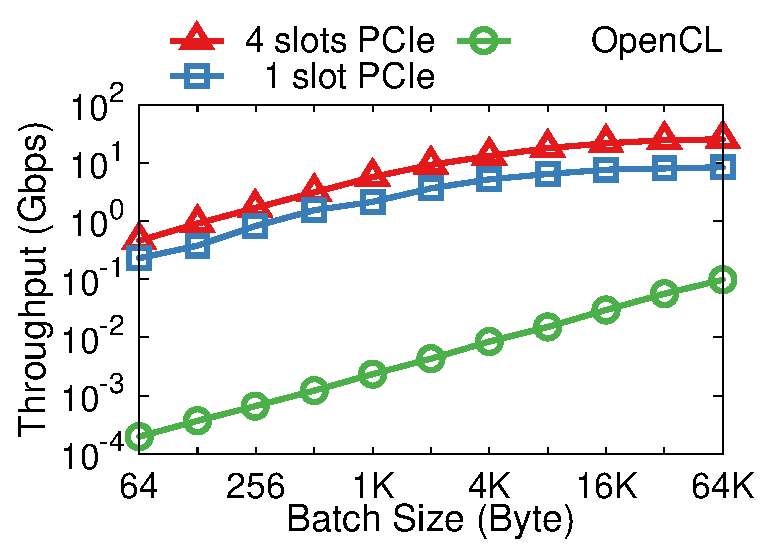
\includegraphics[width=0.5\textwidth]{eval/pcie_1}
	}
	\subfloat[]{
		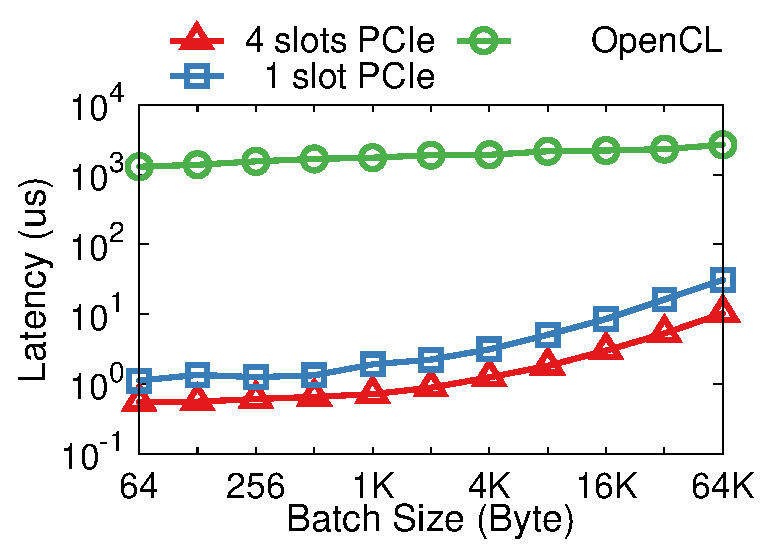
\includegraphics[width=0.5\textwidth]{eval/pcie_2}
	}

	\caption{Performance of PCIe I/O channels. The Y-axis is a logarithmic coordinate system.}

	\label{clicknp:fig:pcie}
\end{figure}

In order to send signals to FPGA components, the \name compiler automatically generates a special component called \textit {CmdHub} in the FPGA.
\textit {CmdHub} distributes the control signals issued by the host management program to FPGA components through pipelines, and the FPGA components return the results of the signal processing functions to \textit {CmdHub} through pipelines, which in turn return to the host management program.
To avoid the complexity of layout and wiring brought about by one-to-many pipeline connections, \textit {CmdHub} forms a daisy chain with all components, starting from \textit {CmdHub}, passing through all components in the topological order of the component connection diagram, and finally returning to \textit {CmdHub}.
In order to identify the target component in the daisy chain, the component ID is embedded in the signal message, and each component only processes the signal message matching the component ID, and directly forwards other signal messages.
 

\subsection{Debugging}
\label{clicknp:subsec:debug}

\name provides two methods for debugging.

\textbf{CPU function simulation.}
\name components are written in class C high-level language, so a component can be compiled into a thread running on the CPU, and the pipeline is the queue between threads. Developers can use familiar software debugging tools for function simulation.



\textbf{Actual FPGA operation.}
CPU function simulation has limitations. Firstly, there is a possibility of deadlock in the communication pipeline between components. During CPU function simulation, due to the inconsistency of timing and hardware logic, deadlock problems may not be discovered; secondly, CPU simulation speed is slow, it cannot reflect actual performance, and it is difficult to test the interaction with PCIe DMA and the network; finally, function simulation cannot discover errors in the compiler. Therefore, in actual applications, after the function simulation passes, it is generally debugged by the method of actual FPGA operation.

Since the variable names in the \name language do not correspond with those in Verilog, online FPGA debugging tools such as SignalTap are not applicable. Therefore, \name requires a customized debugging mechanism. Firstly, in debug mode, \name can record the input and output logs of each pipeline, and transmit them to the host memory via the PCIe I/O pipeline. Secondly, \name allows users to insert printf statements in the component code, and send debug information containing variable values to the host through the pipeline. Thirdly, \name supports users to insert breakpoints at compile time for debugging interactive network protocols or simulating queue blocking leading to deadlock. Breakpoints are compiled into pipeline write operations (notifying the host that the breakpoint has been hit) and blocking read operations (waiting for the host to send the breakpoint continue command). Fourthly, \name allows querying or modifying the value of a variable at any time during operation (including when a breakpoint is hit). When a user queries the value of a variable, a query or modification command is sent through signal, and the value of the variable is returned.

\subsection{Component Hot Migration and High Availability}
\label{subsec:clicknp:fault-tolerance}

Hot migration is a crucial feature that data center network functions need to support. When a virtual machine is hot migrated, the internal state of the corresponding network card on the compute node needs to be hot migrated to the new node, otherwise, it is necessary to reinitialize the network card state on the new node, which brings complexity to the software and migration delay. Similarly, when network and storage nodes are hot migrated due to upgrades, expansions, etc., the network card state also needs to be hot migrated to the new node. In addition, in order to achieve uninterrupted network function upgrades, the internal state needs to be hot migrated to another node, and then the original node is taken offline for upgrades. To achieve high availability, when adding a backup node, in order to synchronize the internal state of the source node and the newly added backup node, hot migration technology is also needed.

The hot migration process commences with the configuration of the switch to stop sending packets to the old FPGA, instead buffering these packets within the switch. The next step involves halting each component within the FPGA through the breakpoint mechanism, as discussed in section \ref{clicknp:subsec:debug}. Following this, all variable values within the components, data in the pipeline, and values in the global memory are exported to the host. The same \name program is then run on the new FPGA, importing the aforementioned internal state of the FPGA through the debugging mechanism, and resuming the operation of each component. Finally, the switch is instructed to modify the routing table, redirecting the address of the old FPGA to the port where the new FPGA is located, and sending the buffered packets in the switch. This concludes the hot migration process.

To ensure high availability of network functions, \name employs the method of state machine replication. Two FPGAs receive the same sequence of packets. Provided there is no randomization or time-related processing logic within the component, and it does not accept control signals from the host, it can be ensured that the internal state of the two FPGAs and the sequence of packets sent out are identical. In the event of a backup node failure, a new backup node is simply initiated, followed by state hot migration. In the event of a primary node failure, a switch to the backup node is necessary. At this point, a small number of input packets may be lost or output packets may be repeated, but these situations can be safely handled by TCP.

\egg{

\egg{
Control signals can only be generated by the manager thread. When the manager thread sends a signal to a target element in FPGA, it embeds the element's ID in the signal message, and passes the message to \textit{CmdHub} through slot 32. \textit{CmdHub} parses the message and forwards the signal request to the corresponding elements, again through FIFO buffers.
}

\egg{
As previously mentioned, OpenCL advocates a batch processing model where communication between the host program and a kernel in FPGA must go through shared DRAM, and the host program cannot control the kernel while it is running. A special kernel could be used to proxy messages between the host program and the kernel via DRAM, but this incurs approximately 1ms latency. DDR access is performed via a PCIe link and raw PCIe latency is merely approximately 1$\mu$s. As we improve kernel communication efficiency with channels in place of shared memory, we design a host-kernel communication mechanism with channel abstraction for low latency and high throughput. We leverage I/O channel in Altera OpenCL and AXI stream in Vivado high-level synthesis to connect the Catapult shell to kernels and build a PCIe bypass switch to arbitrate accesses for on-board DRAM and kernel I/O channel.
}

A PCIe link is divided into multiple logically independent \textit{slots} that can operate simultaneously. One slot is reserved for signals. The remaining slots are allocated to channels between the host and FPGA elements, allowing each channel to transfer data in parallel without head-of-line blocking. On the CPU side, each host element runs on a separate core and receives input flits via PCIe by polling or interrupt. On the FPGA side, each element that communicates with the host is connected to an inbound demultiplexer and an outbound multiplexer, where load-adaptive batching is performed to enhance peak throughput while maintaining low latency under light load.

With the polling model, the latency of the PCIe I/O channel is $< 2 \mu s$ when the message size is small, but the latency can reach up to $32 \mu s$ for fully batched messages. The interrupt model, however, can increase the latency.

Each slot is assigned to one CPU core. Our PCIe channel has two bottlenecks: (1) The PCIe Gen2 x8 interface has a bandwidth of 32 Gbps, and (2) the PCIe data width is 128b, and the clock frequency of the Catapult shell is 200 MHz, which limits the PCIe throughput to 25.6 Gbps. The PCIe I/O channel offers a 1\approx2$\mu$s RTT, which translates to 400\approx800K host-kernel transactions per second. The polling mode provides lower latency and higher throughput, while the latency of the interrupt mode can be improved by utilizing more cores and PCIe slots. Four CPU cores are sufficient to saturate the maximum throughput for both polling and interrupt mode under a 64KB batch size. The effectiveness of batching will be further evaluated in the traffic dumper application.
}
